\phantomsection
\section*{Fuerza Bruta (Naive Algorithm)}
\addcontentsline{toc}{section}{Fuerza Bruta (Naive Algorithm)}

\phantomsection
\subsection*{Introducción al Algoritmo de Fuerza Bruta}
% \addcontentsline{toc}{subsection}{Introducción al Algoritmo de Fuerza Bruta}

\quad El algoritmo de fuerza bruta es un algoritmo que analiza de izquierda a derecha revisando por caracteres si un patrón existe dentro de un texto. Se puede considerar el método más básico de String Matching porque en cada carácter revisa si el patrón se cumple.

\phantomsection
\subsection*{Implementación del Algoritmo de Fuerza Bruta}
(Con ayuda de \cite{coincidenciadecadenasdepython}, \cite{coronadosanz_2018} y \cite{pdfFB})
% \addcontentsline{toc}{subsection}{Implementación del Algoritmo de Fuerza Bruta}
% def fuerza_bruta(txt, patron):
%     N = len(txt)
%     M = len(patron)
%     i = 0   # pointer into the text
%     while i <= (N - M):
%         j = 0       # pointer into the patter
%         while j < M:
%             if txt[i+j] != patron[j]:
%                 break
%             j += 1
%         if j == M:
%             return i
%         i += 1
%     return -1
% \algnewcommand\algorithmicto{\textbf{to}}
% \algrenewtext{For}[3]%
% {\algorithmicfor\ #1 \gets #2 \algorithmicto\ #3 \algorithmicdo}

\begin{algorithm} [H]
    \caption{Algoritmo de fuerza bruta}\label{alg:FB}
    \begin{algorithmic} [1]
        \Procedure{FuerzaBruta}{(texto, patron)}
            \State $n \gets \texttt{len(texto)}$
            \State $m \gets \texttt{len(patron)}$
            \For {$i \leq (n - m)$} \Comment{Despues de $n-m$ no puede ser el patron}
                \For {$j < m$} \Comment{Evalua el patron caracter por caracter}
                    \If {texto[$i + j$] $\neq$ patron[$j$]} \Comment{Evalua si los caracteres son los mismos}
                        \State break
                    \EndIf
                \EndFor
                \If {$j = m$} \Comment{Si llega al final entonces existe y devuelve la posición}
                    \State return $i$
                \EndIf
            \EndFor
            \State return -1 \Comment{Si pasa por todo y no encuentra no existe devuelva -1}
        \EndProcedure
    \end{algorithmic}
\end{algorithm}


\phantomsection
\subsection*{Análisis del Algoritmo de Fuerza Bruta}
% \addcontentsline{toc}{subsection}{Análisis del Algroitmo de Fuerza Bruta}

\subsubsection*{Paso 1: Establecer el tamaño n de los datos}
% \addcontentsline{toc}{subsubsection}{Paso 1: Establecer el tamaño n de los datos}
Hay dos variables que determinan el tamaño de los datos, estos serían $n$ como la cantidad de caracteres del patrón y $m$ la cantidad del texto. Entonces termina siendo $len(patrón) + len(texto) = n + m$

\subsubsection*{Paso 2: Determinar las operaciones de interés}
% \addcontentsline{toc}{subsubsection}{Paso 2: Determinar las operaciones de interés}
Las operaciones de interés del algoritmo son las comparaciones de los caracteres. Estos tendrán valor de 1 cada uno.

\subsubsection*{Paso 3: Encontrar los casos base}
% \addcontentsline{toc}{subsubsection}{Paso 3: Encontrar los casos base}
Este algoritmo implica la combinación de las dos variables de tamaño un tiempo de recorrido del patrón y otro del texto.

\[T_{patrón}(0) =  0\]
\[T_{patrón}(1) = 1\]

\[T_{patrón}(n) = 1 + T_{patrón}(n-1)\]

\[T_{texto}(0) =  0\]
\[T_{texto}(1) = 1\]

\[T_{texto}(m) = 1 + T_{texto}(m-1)\]

y esto se junta para que de (porque para cada caracter del texto se evalúan todos los del patrón):
\[T_{Fuerza Bruta}(n,m) = T_{texto}(m) * T_{patrón}(n)\]

\subsubsection*{Paso 4: Evaluando la ecuación recursiva}
% \addcontentsline{toc}{subsubsection}{Paso 4: Evaluando la ecuación recursiva}

Como es una suma de unos
\[T_{patrón}(n) = 1 + 1 + 1 + 1 ... + 1 + 1\]

\[T_{patrón}(n) = n \]

\[T_{texto}(m) = 1 + 1 + 1 + 1 ... + 1 + 1\]

\[T_{texto}(m) = m \]

Con la ecuación que sacamos en el paso anterior y la evaluación de las sub-ecuaciones entonces llegamos a la conclusión de que:
\[T_{Fuerza Bruta}(n,m) = m*n\]


\subsubsection*{Paso 5: O-grande}
% \addcontentsline{toc}{subsubsection}{Paso 5: O-grande}
Con la ecuación de tiempo entonces concluimos que el O-grande del algoritmo es: $O(n*m)$

\subsubsection*{Paso 6}
% \addcontentsline{toc}{subsubsection}{Paso 6}

\begin{figure} [H]
    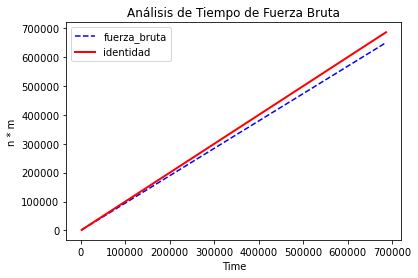
\includegraphics[width=0.45\textwidth]{../codigoPythonJupyter/FuerzaBruta/Final.png}
    \caption{Fuerza Bruta (Apéndice fuerzaBruta.ipynb)}
    \label{fig:fb}
\end{figure}
